\section{The \lang language}

\lang is a minimal ML-like language with
let-polymorphism and abstract types. Its type system manages
linearity and borrows using kinds and (kind-) constrained types.
For ease of presentation, we simplify the language.
\begin{itemize}[topsep=0pt]
\item Pattern matching is demonstrated on pairs rather than algebraic
  datatypes.
\item There are separate operators for borrowing and reborrowing (taking
  the borrow of a borrow).
\item Regions are explicit in the code and must be annotated using the
  algorithms presented in \cref{regionannot}.
\item Regions are identified using nesting levels instead of region
  variables.
\end{itemize}

The rest of this section formalizes  \lang: the syntax (\cref{syntax}),
the statics in terms of a region annotation pass (\cref{regionannot}) and
syntax-directed typing (\cref{sdtyping}),
and a dynamics that is linearity- and resource-aware (\cref{sec:sem}).

\subsection{Syntax}
\label{syntax}

\begin{figure}[!tb]
  \begin{subfigure}[t]{0.45\linewidth}
\begin{align*}
  \htag{Expressions}
  e ::=&\ c \mid x \mid \app{e}{e'} \mid \lam{x}{e} \mid \letin{x}{e}{e'}\\
  % |&\ \fix{e}\tag{Fixpoint}\\
  |&\ \introPair{e}{e'} \mid \matchin{x,y}{e}{e'}\tag{Pairs}\\
  |&\ \region{x}{e}\tag{Region}\\
  |&\ \borrow{x}\tag{Borrows}\\
  % |&\ \introK{K}{e}\tag{Data Constructor introduction}\\
  % |&\ \elimK{K}{e}\tag{Data Constructor elimination}\\
  \htag{Environments}
  \E ::=&\ b^*\\
  b ::=&\ \bvar{x}{\schm}\tag{Variable bindings}\\
  |&\ \bvar{\tvar}{\kschm}\tag{Type bindings}\\
  % |&\ \tydecl{t}{\kschm}{K}{\tau}\tag{Type Declaration}\\
  \htag{Type and kind Schemes}
  \schm ::=&\ \forall\kvar^*\forall\bvar{\alpha}{k}^*.(\qual{C}{\tau})\\
  \kschm ::=&\ \forall\kvar^*.(\qual{C}{k_i^* \karr k})\\
\end{align*}
\end{subfigure}\hfill
\begin{subfigure}[t]{0.5\linewidth}
\begin{align*}
  \htag{Type Expressions}
  \tau ::=&\ \tvar\tag{Type variables}\\
  |&\ \tau\tarr{k}\tau\tag{Function types}\\
  |&\ \tapp{t}{\tau^*}\tag{Type constructors}\\
  |&\ \borrow{\tau}\tag{Borrowed Type}\\
  \htag{Kinds}
  k ::=&\ \kvar\tag{Kind variables}\\
  |&\ \klin_n\tag{Linear kind}\\
  |&\ \kaff_n\tag{Affine kind}\\
  |&\ \kun_n\tag{Unrestricted kind}\\
  n \in&\ \mathbb N \cup \{\infty\}\\
  \htag{Constraints}
  C ::= (\Cleq{k}{k'})^*
\end{align*}
\end{subfigure}

%%% Local Variables:
%%% mode: latex
%%% TeX-master: "main"
%%% End:

  \vspace{-7pt}
  \caption{Syntax}
  \label{grammar}
  \vspace{-10pt}
\end{figure}


\Cref{grammar} defines the syntax of \lang. Expressions are as usual
in an ML-like language.  The novel aspects are match
specifications, regions, and borrows.

A borrow $\borrow{x}$ is always taken from a variable $x$. The
\emph{borrow annotation} $\BORROW$ indicates whether the borrow is exclusive
($\MBORROW$) or shared ($\IBORROW$). If $x$ is already borrowed,
then we need to use the reborrow expression $\reborrow{x}$.
%
A region $\region{\Sone x\BORROW}{e}$ is annotated with its nesting $n$, the variable $x$ that may be borrowed in $e$, and the kind of borrow $\BORROW$.
%
A match is indexed with a \emph{match specification} $\etransfm$ that indicates
whether the match should work on borrows ($\etransfm=\&^b$) or not ($\etransfm=id$).
%
We consider four primitive operations to manipulate resources:
$\create$, $\observe$, $\update$ and $\destroy$.

Many types are indexed with kinds.
A kind $k$ is either a kind variable $\kvar$ or a constant
(linear $\klin$, affine $\kaff$, or unrestricted $\kun$) indexed
by a nesting level $n \in \Nat \cup \{\infty\}$.

A type $\tau$ is either a type variable, a pair type, a function type indexed by a
kind,
a type application $\tapp{\tcon}{\Multi{\tau}}$ of an abstract type constructor
$\T T$, or a borrowed type  $\borrowty{k}{\tau}$.

Type schemes $\schm$ add quantification over kind
variables $\kappa$, kinded type variables $(\alpha:k)$, and constraints
$C$ to a type, where a constraint is a list of inequalities over
kinds.

Abstract type constructors possess kind schemes $\kschm$ which relate
the kinds of the type constructors' arguments to the kind of the
constructed type.

Generally, we write lists with an overbar and (sometimes) an index as
in $\Multi[i]\tau$.

% \paragraph{Previously}


% Let us first define our conventions and meta-syntactic variables.
% Expressions, types and kinds are denoted respectively as $e$, $\tau$, and $k$.
% Variables, type variables and kind variables are denoted
% respectively as $x$, $\tvar$ and $\kvar$. Types and kind schemes
% are denoted by $\schm$ and $\kschm$.
% In the rest of the text, we will write lists with a bar and an index, for
% instance $\Multi[i]{\tau}$.
% Kind constants are denoted in bold capital letters, such as $\kaff$ for affine.

% The syntax of \lang is presented in \cref{grammar} and follows
% traditional ML languages with let bindings.
% Borrows $\borrow{e}$ are annotated with a specification indicating
% if a borrow is immutable ($\IBORROW$) or mutable ($\MBORROW$).
% We also distinguish reborrows, which are written as $\reborrow{e}$.
% Match are indexed with a specification which can be either $\&^b$
% (which $b$ a borrow specification) or $id$, indicating if the match
% should operate on borrows or not.
% Regions $\region{\Sone x\BORROW}{e}$ are annotated with their nesting ($n$)
% and the variable whose borrow they enclose ($x$).
% %
% $\tapp{\tcon}{\Multi{\tau}}$ denotes a type application where
% $\T t$ is an abstract type constructor.
% Arrow and borrow types are annotated with a kind, written as $\tau \tarr{k} \tau$
% and $\borrowty{k}{\tau}$ respectively.
% %
% Kinds can be either a kind variable $\kvar$, or constants
% (linear $\klin$, affine $\kaff$ or unrestricted $\kun$) indexed
% by a nesting level represented by a member of $N \cup \{\infty\}$.
% Type schemes and kind schemes are guarded by a set of constraints.
% %
% Finally, constraints are composed of a list of kind inequalities.

% Environments are composed of value and type bindings, along with type
% declarations. Type declarations, of the form
% $\tydecl{t}{\kschm}{K}{\tau}$, introduce both a new type constructor $\T{t}$ and
% a data constructor $K$.

\subsection{Automatic region annotation}
\label{regionannot}

In \cref{motivation}, region annotations are optional.
In our formalization, regions must be syntactically explicit and annotated with
a nesting index and a scoped variable.
We now define a best-effort
syntactic code transformation $\RannotT{p}{p'}$ which
annotates programs automatically.
The input $p$ is a program with optional region annotations of the form $\region[]{}{e}$.
The output $p'$ is a program with explicit annotations
of the form $\region{\Sone x\BORROW}{e}$.
We give an informal presentation of our code transformation and defer
the complete definition to \cref{appendix:regionannot}. This code transformation
aims to find, for each borrow $\borrow{x}$, the biggest region satisfying
the following rules:
\begin{enumerate}
\item The region should contain at least $\borrow{x}$.
\item The region should never be larger than the scope of $x$.
\item An exclusive borrow $\borrow[\kaff]{x}$ should never share a region with any other borrow of $x$.
\item A use of $x$ can never be in the region of $\borrow{x}$.
\end{enumerate}
We then start from the leaves and grow the region
associated to each borrow until it can't grow anymore either due to a binding
or to conflicting uses. We demonstrate
on the following program:
%
\[
  \setlength{\jot}{-1pt}
  \RannotT{
\begin{aligned}
  \lam{a}{}\ &
  \letin{x}{\app{f}{\borrow[\kun]{a}}}{}\\
  &g\ (\borrow[\kaff]{x});\\
  &f\ (\borrow[\kun]{x})\ (\borrow[\kun]{x})\\
\end{aligned}
}{
\begin{aligned}
  \lam{a}{}\region[1]{\Sone a\MBORROW}{\ &%
  \letin{x}{\app{f}{\borrow[\kaff]{a}}}{}\\
  &\region[2]{\Sone x\MBORROW}{g\ (\borrow[\kaff]{x})};\\
  &\region[2]{\Sone x\IBORROW}{f\ (\borrow[\kun]{x})\ (\borrow[\kun]{x})}\\
  &\!\!\!}
\end{aligned}
}
\]
%
Since $a$ only has one borrow, its region covers its whole lexical scope.
$x$ has multiple conflicting borrows and requires more consideration.
We place a first
region around the exclusive borrow and its function application,
and a second region around both shared borrows. This placement of region
is optimal: making any region bigger would cause a borrowing
error.
Note that indices of regions are well nested, as the inner region have
higher indices than the outer ones.

Programmers might also want to annotate regions explicitly.
Such annotations are considered as
upper bound on the contained regions.
In the following program, a manual annotation has been inserted to ensure
no borrow enters the reference $r$:
%
\[
  \setlength{\jot}{-1pt}
  \RannotT{
\begin{aligned}
  \letin{&r}{\operatorname{ref}\ 0}{}\\
  \lam{a}{}\ &
  set\ r\ \region[]{}{g\ (\borrow[\kun]{a})};\\
  &f\ (\borrow[\kun]{a})
\end{aligned}
}{
\begin{aligned}
  \letin{&r}{\operatorname{ref}\ 0}{}\\
  \lam{a}{}\ &
  set\ r\ \region[1]{\Sone a\IBORROW}{g\ (\borrow[\kun]{a})};\\
  &\region[1]{\Sone a\IBORROW}{f\ (\borrow[\kun]{a})}
\end{aligned}
}
\]
%
The rules allow merging the two regions around the borrows
$\borrow[\kun]{a}$. However
the explicit annotation indicates that the region should stay around the closure
passed as argument of $set$. This is useful to control captures
by imperative APIs.

This code transformation is purely syntactic and must be used before
typing. It only produces well-nested annotations: if $\region[n]{b}{\dots}$
is nested inside $\region[n']{b'}{\dots}$, then $n > n'$. Furthermore, there
is at most one region per borrow, and exactly one region per exclusive borrow.
In the rest of this article, we consider
that all terms have been annotated with this code transformation and respect
these properties.

\subsection{Typing}
\label{sdtyping}

We now focus on the essential and novel parts of the type system. A complete
description is available in \cref{appendix:sdtyping}.
% In this section, we focus on chosen parts of our system
% through a set of selected rules.
%
We discuss the following judgments:
\begin{description}
\item[$\inferS{C}{\E}{e}{\tau}$ --]
  Expression $e$ has type $\tau$ in environment $\E$ under constraints $C$.
\item[$\inferSK{C}{\E}{\tau}{k}$ --]
  Type $\tau$ has kind $k$ in environment $\E$ under constraints $C$.
\item[$\entail{D}{C}$ --] Constraint $D$ entails constraint $C$.
\end{description}

\paragraph{Kinds and constraints}

\affe uses kinds and constrained types to indicate
linear and affine types.
% Before explaining the details of our type system, we
% give a quick presentation of the kinds and constraints.
A kind $k$ is either a kind variable, $\kvar$, or a constant $\mul_n$.
The quality $\mul$ describes the use pattern of the type:
unrestricted $\kun$, affine $\kaff$, or linear $\klin$. The level $n \in \Nat \cup \{\infty\}$
describes the nested regions in which the value can be used.
Level $0$ refers to the top-level scope outside any region; we often elide it
and write $\kaff$ for $\kaff_0$. Level
$\infty$ refers to an empty region that is infinitely nested.
For instance, the constraint $\Cleq{\kvar}{\kun_\infty}$ indicates that
$\kvar$ must be unrestricted, but can be local to a region.
%
Kinds form a lattice described in \cref{sdtyp:lattice}.
Unrestricted values may be used
where affine ones are expected and affine ones are less restricted
than linear ones as reflected in \TirName{Lat-UAL}.
Values usable at level $n$ may be used at any more deeply
nested level $n'$ as defined in the \TirName{Lat-Level} axioms.
%
Constraints are conjunctions of inequality constraints over this kind
lattice. In most uses, constraints give upper or lower bounds for
kind variables or relate two kind variables.

\begin{figure}[tp]
  \begin{minipage}{0.65\linewidth}
  \begin{mathpar}
    \inferrule[Lat-UAL]{}{\kun \lk \kaff \lk \klin}
    \and
    \inferrule[Lat-Level]{\mul \lk \mul' \and n \lk n'}{\mul_n \lk_\Lat \mul'_{n'}}
  \end{mathpar}
\end{minipage}~
\begin{minipage}{0.2\linewidth}
  \centering
  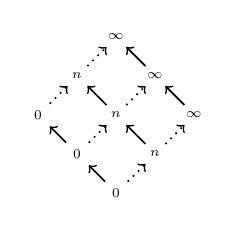
\begin{tikzpicture}
    [->,auto,semithick, every node/.style={scale=0.7}]
    \node(U) {$\kun_0$} ;
    \node(A) [above left of=U] {$\kaff_0$} ;
    \node(L) [above left of=A] {$\klin_0$} ;
    \node(Un) [above right of=U] {$\kun_n$} ;
    \node(An) [above left of=Un] {$\kaff_n$} ;
    \node(Ln) [above left of=An] {$\klin_n$} ;
    \node(Uinf) [above right of=Un] {$\kun_\infty$} ;
    \node(Ainf) [above left of=Uinf] {$\kaff_\infty$} ;
    \node(Linf) [above left of=Ainf] {$\klin_\infty$} ;
    \path
    (U) edge (A)
    (A) edge (L)
    (Un) edge (An)
    (An) edge (Ln)
    (Uinf) edge (Ainf)
    (Ainf) edge (Linf)
    ;
    \path[dotted]
    (U) edge (Un)
    (A) edge (An)
    (L) edge (Ln)
    (Un) edge (Uinf)
    (An) edge (Ainf)
    (Ln) edge (Linf)
    ;
  \end{tikzpicture}
\end{minipage}

%%% Local Variables:
%%% mode: latex
%%% TeX-master: "../main"
%%% End:

  \vspace{-10pt}
  \caption{Lattice ordering -- $k \lk_\Lat k'$}
  \label{sdtyp:lattice}
  \vspace{-10pt}
\end{figure}

\paragraph{Environments and bindings}
\label{sdtyping:envs}

\begin{figure}[tp]
  \begin{minipage}{0.36\linewidth}
  \begin{align*}
    \E ::=&\ \Eempty \mid \E;B\tag{Environments}\\
    B ::=&\ \bnone \tag{Empty} \\
    |&\ \bvar{\tvar}{\kschm} \tag{Types}\\
    |&\ \bvar{x}{\schm} \tag{Variables} \\
    |&\ \bvar{\borrow{x}}{\borrowty{k}{\tau}} \tag{Borrows}\\
    |&\ \svar{x}{\schm}^n \tag{Suspended}
    % |&\ \tydecl{t}{\kschm}{K}{\tau}\tag{Type Declaration}\\
  \end{align*}
  \vspace{-10pt}
  \caption{Type environments}
  \label{grammar:env}
  \end{minipage}\hfill
  \begin{minipage}{0.6\linewidth}
    \begin{tabular}
  {@{}>{$}r<{$}@{ $\vdash_e$ }
  >{$}c<{$}@{ $=$ }
  >{$}c<{$}@{ $\ltimes$ }
  >{$}c<{$}r}

  \Cleq{\schm}{\kun_\infty}
  &\bvar{x}{\schm}&\bvar{x}{\schm}&\bvar{x}{\schm}
  &(Both)\\

  {\Cempty}&
             {\bbvar[\IBORROW]{x} k \schm}&
                                            \bbvar[\IBORROW]{x}
                                            k{\schm}&{\bbvar[\IBORROW]{x}
                                                      k {\schm}}
  &(Borrow)
  % \\
  
  % {\Cempty}&
  % \svar[\IBORROW]{x}{\schm}^n&\svar[\IBORROW]{x}{\schm}^n&\svar[\IBORROW]{x}{\schm}^n
  % &BothS
  \\[2mm]

  {\Cempty}&{B_x}&{B_x}&{\bnone}
  &(Left)\\
  {\Cempty}&{B_x}&{\bnone}&{B_x}
  &(Right)\\[2mm]

  {\Cempty}&{\bvar x \schm}&{\svar x \schm^n}&{\bvar x \schm}
  &(Susp)\\

  {\Cempty}&
             {\bbvar x k \schm}&{\svar[\IBORROW] x \schm^n}&{\bbvar x k \schm}
  &(SuspB)\\

  {\Cempty}&
             {\svar{x} \schm^{n'}}&{\svar[\IBORROW] x \schm^n}&{\svar{x} \schm^{n'}}
  &(SuspS)\\
\end{tabular}
%%% Local Variables:
%%% mode: latex
%%% TeX-master: "../main"
%%% End:

    \vspace{-5pt}
    \caption{Splitting rules for bindings -- $\lsplit{C}{B}{B_l}{B_r}$}
    \label{sdtyp:split}
  \end{minipage}
\end{figure}


\begin{figure*}[tp]
  % \begin{minipage}{0.7\linewidth}
    \begin{mathpar}
      \ruleSDVar
      \and
      \ruleSDApp
      \and
      \ruleSDRegion
      \and
      \ruleSDBorrow
      \and
      \ruleSDLam
      \and
      \inferrule[BorrowBinding]{
        \entail{C}{(\BORROW_n\lk k) \wedge (k \lk \BORROW_\infty)}\\
        \BORROW\in\left\{\kun,\kaff\right\}
      }{
        \lregion{C}{}
        {\svar[\BORROW]{x}{\tau}^n}
        {\bvar{\borrow[\BORROW]{x}}{\borrowty[\BORROW] k{\tau}}}
      }
      % \and
      % \ruleSDPair
      % \and
      % \ruleSDMatchPair
    \end{mathpar}
    \vspace{-10pt}
    \caption{Selected typing rules ($\inferS{C}{\E}{e}{\tau}$)
      and borrowing rules ($\lregion{C}{x}{\E}{\E'}$)}
    \label{selectrules:borrow}
    \label{selectrules:binders}
    \label{sdtyp:app}
    \label{selectrules:region}
    \label{env:rule:borrow}
    \vspace{-5pt}
  % \end{minipage}
\end{figure*}

\lang controls the use of variables by supporting new modes of
binding in type environments $\E$, as defined in \cref{grammar:env}.
Environments contain standard bindings of type variables to kind schemes,
$\bvar{\tvar}{\kschm}$, value bindings $\bvar{x}{\schm}$, but also
suspended and borrow bindings.
A suspended binding, $\svar{x}{\schm}^n$, indicates that $x$ is
earmarked for a borrowing use in a nested region
marked with $x$ % (see \cref{sdtyping:regions}),
but
cannot be used directly.
A borrow binding, $\bvar{\borrow{x}}{\borrowty{k}{\schm}}$, replaces
such a suspended binding on entry to the $x$-region. It indicates
that the borrow $\borrow{x}$ can be used directly. Kind $k$
restricts the lifetime of the borrow to the region (see \cref{selectrules:borrow}).

% , either
% through
% linearity and affinity which restrict how variables are shared and ignored,
% or through borrows which allow to circumvent the linearity rules
% in a controlled way.
% In order to check these properties, we introduce several new bindings
% in our typing environments.
% The grammar of type environment (denoted $\E$) is shown in \cref{grammar:env}.

% Environments are also used to encode several linearity-related properties
% through \emph{environment-wide constraints}.
Constraints on an environment control substructural properties by
restricting the types of variables.  The constraint $\Cleq{\E}{k}$
abbreviates $\Cleq\schm k$, for all $\bvar{x}{\schm}$
% $\svar{x}\schm$, and $\bvar{\borrow{x}}{\borrowty{k'}{\schm}}$
in $\E$, which in turn means that $k' \lk k$ where $k'$ is the kind of
the variable's type scheme.
Borrow bindings follow the exact same rules, but suspended bindings
are forbidden in an environment $\E$ constrained like that.
This intuitive explanation is sufficient to understand
the {\sc Abs} and {\sc Var} rules shown in
\cref{selectrules:binders}.

Rule {\sc Var} looks up the type scheme of the variable $x$ in
the environment $\E$
and instantiates it using the substitution $\unif$. The rule also
checks that the other bindings in $\E$ can be safely discarded by
imposing the constraint $\Cleq{\E\Sdel{x}}{\kaff_\infty}$.
It enforces that all remaining bindings (except $x$) are affine or
unrestricted and can therefore be discarded.

Rule {\sc Abs} ensures the kind annotation on the arrow type
($\tau_2 \tarr{k} \tau_1$) reflects the restrictions on captured variables
via the constraint $\Cleq\E k$.
If, for instance, any binding in $\E$ is affine, it gives rise to the
constraint $\Cleq{\kaff_n}{k}$ and the arrow kind is at least
affine at nesting level $n$.
Capturing a borrow is perfectly fine: the kind of the borrow is also a
lower bound of the arrow kind $k$ which restricts the closure
to the region of the borrow.
Capturing a suspended binding is forbidden.
% Note that $x$ is \emph{not} included in $\E$: since it's the argument of the
% closure, its use should not induce a capture.




\paragraph{Copying and Splitting}
\label{sdtyping:split}

The {\sc App} typing rule in \cref{sdtyp:app} demonstrates how \lang
deals with duplication and dropping of values.
The splitting $\lsplit{C}{\E}{\E_1}{\E_2}$ in the rule decomposes the
type environment $\E$ in two parts, $\E_1$ and $\E_2$, which are used
to typecheck the components of the application.
% The constraint $C$ characterizes a valid  splitting.

\cref{sdtyp:split} shows the action of splitting rules on single
bindings. If $x$'s type is unrestricted,
rule {\sc Both} indicates that we can duplicate it.
Similarly, unrestricted borrows can be duplicated with rule
{\sc Borrow}.
{\sc Left} and {\sc Right} rules are always applicable and move a binding
either to the left or right environment.
The rules {\sc Susp}, {\sc SuspB} and {\sc SuspS}
split off suspended bindings to
the left while conserving access to the binding on the right.
A suspended binding can later be turned
into a borrow inside a region. Splitting of suspended bindings is
asymmetric. It must follow the order of execution from left to right,
which means that a resource can be used first as a borrow on the left
and then later as a full resource on the right. The {\sc Susp} rule
works with a full resource, the {\sc SuspB}
with a borrow and {\sc SuspS} with a suspended binding.

Splitting applies whenever an
expression has multiple subexpressions:  function applications,
let bindings and pairs. In the
expression
$\letin{a}{\text{create}\ 8\ x}
{f\ \region[{}]{\Sone a\IBORROW}{\text{length}\ \borrow[\IBORROW]{a}}\ a}$,
the rule {\sc Susp} splits off a borrow from  the resource
$a$ to use it in the left argument.
As usual, a borrow cannot be active in the same scope as its resource.
The \emph{region} around its use ensures that the borrow in the left argument
does not
escape, which brings us to the next topic.

\paragraph{Regions}
\label{sdtyping:regions}

% \begin{figure}[tp]
%   % \begin{minipage}{0.4\linewidth}
%   %   \centering
%   %   \begin{mathpar}
%   %     \ruleSDRegion
%   %   \end{mathpar}
%   %   \caption{The {\sc Region} rule}
%   %   \label{selectrules:region}
%   % \end{minipage}\hfill
%   % \begin{minipage}{\linewidth}
%     \centering
%     % \begin{tabular}
%     %   {@{}>{$}r<{$}@{ $\vdash_e$ }
%     %   >{$}c<{$}@{ $\rightsquigarrow_n^{x}$ }
%     %   >{$}l<{$}
%     %   r}

%     %   (\kun_n\lk k\lk\kun_\infty)
%     %   &{\svar[\IBORROW]{x}{\tau}^n}
%     %   &{\bvar{\borrow[\IBORROW]{x}}{\borrowty[\IBORROW] k{\tau}}}
%     %   &Immut\\

%     %   (\kaff_n\lk k\lk\kaff_\infty)
%     %   &\svar[\MBORROW]{x}{\tau}^n
%     %   &\bvar{\borrow[\MBORROW]{x}}{\borrowty[\MBORROW] k{\tau}}
%     %   &Mut
%     % \end{tabular}
%     \begin{mathpar}
%     \end{mathpar}
%     \vspace{-10pt}
%     \caption{Borrowing rules for bindings -- }
%   \vspace{-10pt}
%   % \end{minipage}
% \end{figure}

Borrowing is crucial to support an imperative programming style.
To guarantee the validity of a borrow, its lifetime must be properly contained in its
ancestor's lifetime. \lang ensures proper nesting of lifetimes by using
regions. The expression $\region{\Sone x\BORROW}{e}$ indicates a
region at nesting level $n$ in which a $\BORROW$-borrow can be taken of $x$.

The typing for a region (rule {\sc Region} in \cref{selectrules:region})
replaces suspended bindings by borrow bindings
(rule {\sc BorrowBinding}), typechecks the body
of the region, and ensures that the borrow does not leak outside.
This last check is done with indices that correspond to the nesting
level of the region. The kind $k$ of the borrow is indexed with the level $n$
corresponding to its region, thanks to the constraint $(\BORROW_n\lk
k)$. The constraint $\Cleq{\tau}{\klin_{n-1}}$ ensures that
the return type of the region must live at some enclosing, lower level.

As an example, consider the expression $\region{\Sone x\IBORROW}{f(\borrow[\IBORROW]{c})}$
where $c$ is a linear channel in an environment $\E$.
The first step is to check that $\svar[\IBORROW]{c}{\text{channel}}$
is in $\E$.
When entering the region, rule \TirName{Region} imposes
$\lregion{C}{x}{\E}{\E'}$, which defines $\E'$
corresponding to $\E$ where the suspended binding is replaced by the
borrow binding  $\bvar{\borrow[\IBORROW]{c}}{\borrowty[\IBORROW]{k}{\text{channel}}}$.
To constrain the borrow to this region we impose the constraint
$\entail{C}{(\kun_n\lk k) \wedge (k \lk\kun_\infty)}$, which affirms
that the borrow is unrestricted, but can only be used in nesting
levels $n$ and higher.
%
% With that setup we typecheck the body of the region,
% $f(\borrow[\IBORROW]{c})$.
% The constraint $\Cleq{\tau}{\klin_{n-1}}$ ensures
% that the kind of $\tau$ does not contain anything whose kind is
% ``above level $n$'' and thus confines the borrow to the region
% (for instance, $\borrowty[\IBORROW]{\kun_n}{\text{c}}$ has kind
% $\kun_n$ and thus cannot be returned).
%
Rule {\sc Region} also imposes the constraint
$\Cleq{\tau}{\klin_{n-1}}$, which prevents the borrow, having kind $k$ of level
$\geq n$, from escaping the region's body of type $\tau$.


% As it would be cumbersome to markup regions manually, we developed an
% algorithm that starts from each borrow, creates a region around it,
% and extends it as much as possible while respecting other borrows
% and binders. The algorithm (see \cref{regionannot}) also provides the region's level
% and variable annotation.
% Henceforth, we consider terms with fully annotated regions.



% \paragraph{Kind checking}

% \TODO{Present this if we have enough space}


\paragraph{Pattern matching}
\label{sdtyping:matching}

Elimination of pairs is done using a matching construct
$(\matchin{x,x'}{e_1}{e_2})$.
This construct is mostly standard, except it can operate both
on normal pairs and borrows of pairs.
The intuition is as follow:
A syntactic marker $\etransfm$ indicates if it applies to
a pair ($\etransfm = \operatorname{id}$) or a borrow ($\etransfm = \&^\BORROW$).
If $\etransfm = \operatorname{id}$, the typing simplifies to
a regular destruct on pairs.
Otherwise, $e_1$ is expected to be of type
$\borrowty{k}{\tyPair{\tau_1}{\tau'_1}}$
while $x$ and $x'$ are of type respectively
$\borrowty{k}{\tau_1}$ and $\borrowty{k}{\tau'_1}$.

% Matching is voluntarily simple here and
% could be improved using a richer pattern language
% to access inner components and a typeclass mechanisms
% to avoid the need for explicit markers for borrow matches.
% Both extensions are compatible with our system and have been partially
% implemented in our prototype type-checker.


\paragraph{Resource management}

As a model of resource, we consider a simple abstract
type $\tapp{\tres}{\tau}$ whose content of type $\tau$ must be $\kun_0$ and
equipped with the four class of operations describe in \cref{motivation}:
\begin{itemize}[topsep=0pt]
\item
$\create$:
$\forall{\kvar_\tvar}\bvar{\tvar}{\kvar_\tvar}.\
\qual{\Cleq {\kvar_\tvar} {\kun_0}}
{\tvar \tarr{} \tapp\tres\tvar}$
% Creates a new resource.
\item
$\observe$:
$\forall{\kvar\kvar_\tvar}\bvar{\tvar}{\kvar_\tvar}.\
\qual{\Cleq {\kvar_\tvar} {\kun_0}}
{\borrowty[\IBORROW]{\kvar}{\tapp\tres\tvar} \tarr{} \tvar}$
% Reads from a shared borrow of a resource.
\item
$\update$:
$\forall{\kvar\kvar_\tvar}\bvar{\tvar}{\kvar_\tvar}.\
\qual{\Cleq {\kvar_\tvar} {\kun_0}}
\borrowty[\MBORROW]{\kvar}{\tapp\tres\tvar} \tarr{} \tvar \tarr{\kaff} \tunit$
% Writes to an exclusive borrow of a resource.
\item
$\destroy$:
$\forall{\kvar_\tvar}\bvar{\tvar}{\kvar_\tvar}.\
\qual{\Cleq {\kvar_\tvar} {\kun_0}}
\tapp\tres\tvar \tarr{} \tunit$
% Destroys a resource.
\end{itemize}

% \clearpage
\subsection{Semantics}
\label{sec:sem}
\begin{figure}[!tbp]
%   \begin{align*}
% \end{align*}
% \begin{minipage}[t]{0.49\linewidth}
  \begin{align*}
    \htag{Elaborated expressions}
    v ::=~& x \mid \ivar x {\Multi k} {\Multi\tau} \mid \lam[k]{x}{e} \mid \introPair[k]{v}{v'}\\
    e ::=~& x \mid \ivar x {\Multi k} {\Multi\tau} \mid \lam[k]{x}{e} \mid \introPair[k]{e}{e'}\\
    \mid~& \matchin{x,y}{e}{e'} \tag{Tagged pairs}\\
    \mid~& \letin{x}{e}{e'}\\
    \mid~& \letin{\bvar x \schm}{v}{e'}\\
    \mid~& \iapp{\Sp}{e}{e'} \tag{El. application}\\
    \mid~& \region{\Sone x\BORROW}{e}\tag{Region}\\
    \mid~& \borrow{x} \mid \reborrow{x}\tag{Borrows}\\
    \mid~& \create \mid \observe \mid \update \mid \destroy \tag{Resources}\\
    % e &::= \dots \\
    % &\mid \ilam{\Multi\kvar}{\Multi{\tvar : k}}Ckx{\tau}e \tag{El. poly abstraction} \\
    % &\mid \imlam kx{\tau}e \tag{El. mono abstraction} \\
    % &\mid \ivar x {\Multi k} {\Multi\tau} \tag{Instantiation} \\
    % &\mid \introPair[k]{e}{e} \tag{Tagged pairs}\\
    % &\mid \iapp{\Sp}{e}{e} \tag{El. application}\\
    \htag{Elaborated A-normal expressions}
    % TODO: what about constructors applied to values?
    X ::=~& x \mid \ivar x {\Multi k} {\Multi\tau}\\
    v ::=~& c \mid X \mid \lam[k]{x}{e} \mid \introPair[k]{X}{X'}\\
    E ::=~& c \mid X \mid \lam[k]{x}{e} \mid \introPair[k]{x}{x'}\\
    \mid~& \borrow{x} \mid \reborrow{x}\tag{Borrows}\\
    \mid~& \create \mid \observe \mid \update \mid \destroy \tag{Resources}\\
    \mid~& \app{x}{x'} \tag{El. application}\\
    e ::=~& \letin{x}{E}{e'}\\
    \mid~& \letin{\bvar x \schm}{v}{e'}\\
    \mid~& \matchin{x,y}{z}{e} \tag{Tagged pairs}\\
    \mid~& \region{\Sone x\BORROW}{e}\tag{Region}\\
    \htag{Environment}
    \Addr ::=~& \Multi\IBORROW\Multi\MBORROW\Loc \tag{Locations}
    % \\           &\mid \borrow{\Addr} \tag{Borrows}
    \\
    \Perm ::=~& \{\} \mid \Perm + \Addr \tag{Permissions}
    \\
    r ::=~& \Addr \mid c \tag{Results}\\
    \VEnv ::=~& \Eempty \mid \VEnv( x \mapsto r) \tag{Enviroments} \\
%   \end{align*}
% \end{minipage}
% \hfill
% \begin{minipage}[t]{0.49\linewidth}
%   \begin{align*}
    \htag{Storables}
    w ::=~& \StPClosure \VEnv {\Multi\kvar} C k x e \tag{Poly Closures}\\
    \mid~& \StClosure \VEnv k x e \tag{Closures} \\
    \mid~& \StPair k r r \tag{Pairs} \\
    \mid~& \StRes r \tag{Resources} \\
    \mid~& \StFreed \tag{Freed Resource}
    \\
    \htag{Store}
    \Store ::=~& \Eempty \mid \Store( \Loc \mapsto w)
    \\
    \htag{Splittings}
    \Sp ::=~& \Multi{\SpBoth \mid \SpBorrow \mid \SpLeft \mid \SpRight \mid \SpSusp \mid \SpSuspB}
  \end{align*}
% \end{minipage}
\caption{Syntax of internal language}
\label{fig:syntax-internal-language}
\end{figure}

%%% Local Variables:
%%% mode: latex
%%% TeX-master: "main"
%%% End:


\lstMakeShortInline[keepspaces,style=rule,basicstyle=\normalsize\normalfont]@

The dynamics of \lang is given in big-step
functional
style~\cite{siek13:_type_safet_three_easy_lemmas,DBLP:conf/esop/OwensMKT16,
  DBLP:conf/popl/AminR17}.  A function
@eval \Store \Perm \VEnv i e@
manipulates the semantic objects defined in
\cref{fig:syntax-internal-language}.
% To demonstrate resource handling, the semantics comes with an abstract
% notion of linear resources that can be created, destroyed, observed
% (through unrestricted borrows), and
% updated (through affine borrows).
%
The semantics is defined in terms of \emph{elaborated expressions} $e$
with kind, constraint, and splitting annotations inserted by the typechecker.
A splitting $\Sp$ is evidence of the splitting relation for type environments
used in the typing rules.

Let-polymorphism is demonstrated for functions giving rise to elaborated
$\eletfun$ expressions annotated with a type scheme $\schm$ and a kind $k$ indicating their
usage restriction (linear, affine, etc) relative to the variables and
constraints of $\schm$. Their use
gives rise to explicit instantiation of the kind and type variables.
Pairs come with a kind tag $k$ indicating the usage restriction.

Addresses $\Addr$ are composed of a raw location $\Loc$, which is just
a pointer into a store, and a stack of modifiers that indicates the
borrows that have been taken from the original object. From the raw
location, we may take affine borrows and reborrows. Once we have
taken an unrestricted borrow (from a raw location or a borrowed one),
then we can take further unrestricted borrows from it, but no more
affine ones.

A permission $\Perm$ is a set of addresses that may be accessed during
evaluation. A well-formed permission contains at most one address for each raw
location.

Non-trivial results are boxed in the  semantics. So, a result
$r$ is either an address or a primitive constant (e.g., a number).

A value environment $\VEnv$  maps variables to results.

A storable $w$ describes the content of a location in the store. There are five
kinds of storables. A \emph{poly closure} represents a polymorphic
function. It consists of an environment and the components of an
elaborated abstraction. A \emph{closure} represents a monomorphic
function in the usual way.
% A \emph{pair}
% consists of a kind and two results.
A \emph{resource} contains
a result and the \emph{hole} $\StFreed$ fills a released location.

A store $\Store$ is a partial map from raw locations to
storables. The function
@salloc: store -> storable -> (loc * store)@ is such that
@salloc delta@ @w@ allocates an unused location in @delta@ and fills it with
@w@. It returns the location and the extended store.


The evaluation function is indexed by a step count @i@ so that each
invocation is guaranteed to terminate either with an error, a timeout,
or a result. Its return type is a monad
@'a sem@ which combines error reporting and timeout:
\begin{lstlisting}
type 'a sem = Error of string | TimeOut | Ok of 'a
val eval: store->perm->venv->int->exp->(store*perm*result) sem
\end{lstlisting}
It evaluates the given expression in the context of an initial store, a
permission to use addresses in the store, a value environment, and a
step count. If successful, it returns the final store, the remaining
permissions, and the actual result.

\begin{figure}
  \lstsemrule{varinst}
  \medskip
  \lstsemrule{sapp}
  \medskip
  \lstsemrule{spair}
  \medskip
  \lstsemrule{sregion}
  \caption{Big-step Interpretation}
\end{figure}


%%% Local Variables:
%%% mode: latex
%%% TeX-master: "main"
%%% End:


We give some excerpts of the definition of @eval@ in
\cref{fig:big-step-interpretation} and leave the full
definition for \cref{sec:semant-defin}.
% The appendix also
% contains the semantics in mathematical notation.
The definition uses OCaml syntax with some pretty
printing. The pervasive @let*@ operator acts as monadic bind
for the @sem@ monad. The operator
@let*? : bool -> (unit -> 'a sem) -> 'a sem@
 converts a boolean
argument into success or failure in the monad.
 The function header of @eval@ checks
whether time is up and otherwise proceeds processing the expression.

The @Varinst@ case corresponds to instantiation. It
obtains the variable's value, checks that it is a location, checks the
permission (the @let*?@ clause), obtains the storable $w$ at that
location, and checks that it is a poly closure (STPOLY). Next, it updates the
permission: if the poly closure is unrestricted, then the location
remains in the permission set, otherwise it is removed. Finally, we
allocate a new monomorphic closure, add it to the permissions, and
return the pointer as the result along with the updated store and
permissions.

The @App@ case implements (elaborated) function application.
We first apply the splitting @sp@ to @gamma@ and
evaluate subterm @e_1@ with its part of the environment and the
decremented timer @i'@. The result must be a location that we are
permitted to use. Moreover, there must be a monomorphic STCLOS stored
at that location. The permission to further use this closure  remains
in force only if the closure is unrestricted. Finally, we evaluate the
argument, then the function body, and return its result.

% The @Pair@ case corresponds to the \TirName{Pair} typing rule. It
% requires no new features.


The @Region@ case implements a region. It obtains the address for @x@,
the suspended binding, and extends it with the intended borrow
$\BORROW$. This extension may fail if we try to take an affine borrow
of an unrestricted borrow. Next, we rebind @x@ to the borrow's
address, extend the permission accordingly, and execute the region's
body.  Finally, we withdraw the permission and return the result.

The @Borrow@ case obtains the address for @x@, checks that it is a
borrow of the correct mode $\BORROW$ and whether it is permitted to
use it. It just returns the address.

\lstDeleteShortInline@

%%% Local Variables:
%%% mode: latex
%%% TeX-master: "main"
%%% End:
